\documentclass[10pt,conference,compsocconf,letterpaper]{IEEEtran}
%\documentclass[10pt,pdftex,a4paper]{article}%
%\documentclass{sig-alt-release2}
%\documentclass{llncs}
%\usepackage{llncsdoc}
\usepackage{float}
\usepackage{float}
% \floatstyle{boxed}
% \restylefloat{figure}

\usepackage{subfig}
\usepackage{verbatim} 
\usepackage{amssymb}
\usepackage{lipsum}
\usepackage{multicol}
\usepackage{amsmath}
\usepackage{color}
\usepackage{framed}
\usepackage{hyperref}
\usepackage{macros}
\usepackage{url}
\usepackage{xspace}
\usepackage{xifthen}
\usepackage{listings}
%\usepackage{amsthm}
\usepackage{cite}
\usepackage{paralist}
\usepackage{comment}
\usepackage{parcolumns}
\usepackage{fancyvrb}
\usepackage[draft]{fixme}
\newif\ifcode
\codefalse
%%%
% comment this if you do not have
% algpseudocode package for algorithms.
\codetrue
%%%
%\usepackage{macros}
\ifcode
\usepackage[linesnumbered, ruled]{algorithm2e}
\usepackage{algpseudocode}
\usepackage{ioa_code}

\ifx\pdftexversion\undefined
  \usepackage[dvips]{graphicx}
\else
  \usepackage[pdftex]{graphicx}
  \DeclareGraphicsRule{*}{mps}{*}{}
\fi

\PassOptionsToPackage{pdftex}{graphicx}
\usepackage{tikz}

\usepackage{cleveref}
\crefname{section}{\S}{\S\S}
\newcommand{\RNum}[1]{\uppercase\expandafter{\romannumeral #1\relax}}
%%%%%%%%%%%%%%%%%%%%%%%%%%%%%%%%%%%%%%%%%%%%%%%%%%%%%%%%%%%%%%%%%%%%%%%%%=
%%%%%%%%%%%%%%%%%%%%%%%%%%
%pour avoir plus de place
% \topmargin 0pt
% \advance \topmargin by -\headheight
% \advance \topmargin by -\headsep
% \textheight 8.9in
% \oddsidemargin 0pt
% \evensidemargin \oddsidemargin
% \marginparwidth 0.5in
% \textwidth 6.5in
% \setlength{\baselineskip}{13.2pt} % standard value is 13.75pt
\def\algofont{\footnotesize} %fonte pour les algos
%\interfootnotelinepenalty=10
%fin de pour avoir plus de place
%du coup il faut commenter la suite
%\textwidth 130mm
%\textheight 215mm
%jusqu'ici
%\renewcommand{\baselinestretch}{1.5}

%%%%%%%%%%%%%%%%%%%%%%%%%%%%%%%%%%%%%%%%%%%%%%%%%%%%%%%%%%%%%%%%
% Definitions
%%%%%%%%%%%%%%%%%%%%%%%%%%%%%%%%%%%%%%%%%%%%%%%%%%%%%%%%%%%%%%%%

\newtheorem{theorem}{Theorem}
%\newtheorem{reptheorem}[]{Theorem \ref{th:sl}}
%\newreptheorem{theorem}{Theorem}
\newtheorem{axiom}[theorem]{Axiom}
\newtheorem{case}[theorem]{Case}
\newtheorem{claim}[theorem]{Claim}
\newtheorem{proposition}{Proposition}
\newtheorem{explanation}[theorem]{Explanation}
\newtheorem{remark}[theorem]{Remark}
\newtheorem{fact}[theorem]{Fact}
% \newtheorem{conclusion}[theorem]{Conclusion}
% \newtheorem{condition}[theorem]{Condition}
\newtheorem{conjecture}[theorem]{Conjecture}
\newtheorem{corollary}[theorem]{Corollary}
% \newtheorem{criterion}[theorem]{Criterion}
\newtheorem{definition}{Definition}
% \newtheorem{exercise}[theorem]{Exercise}
\newtheorem{lemma}[theorem]{Lemma}
% \newtheorem{notation}[theorem]{Notation}
% \newtheorem{problem}[theorem]{Problem}
%\newtheorem{proposition}[theorem]{Proposition}
% \newtheorem{remark}[theorem]{Remark}
% \newtheorem{solution}[theorem]{Solution}
% \newtheorem{summary}[theorem]{Summary}
\newtheorem{observation}[theorem]{Observation}
%\newenvironment{proof}[1][Proof]{\noindent\textbf{#1.} }{\hfill $\Box$\\[2mm]} %\rule{0.5em}{0.5em}\\}
%\newenvironment{proofsketch}[1][Proof sketch]{\noindent\textbf{#1.} }{\hfill $\Box$\\[2mm]} %\rule{0.5em}{0.5em}\\}
\newenvironment{proofsketch}[1][Proof sketch]{\noindent\textbf{#1.} }{\hfill $\Box$\\[2mm]}

\newenvironment{reptheorem}[1][Theorem]{\noindent\textbf{#1}}{}
\def\lf{\tiny}
\def\rrnnll{\setcounter{linenumber}{0}}
\def\nnll{\refstepcounter{linenumber}\lf\thelinenumber}
\newcounter{linenumber}
\newenvironment{algorithmfig}{\hrule\vskip 3mm}{ \vskip 3mm \hrule }

\def\P{\ensuremath{\mathcal{P}}}
\def\DP{\ensuremath{\Diamond\mathcal{P}}}
\def\DS{\ensuremath{\Diamond\mathcal{S}}}
%\def\T{\ensuremath{\mathcal{T}}}
\def\Time{\mathbb{T}}
%\def\S{\ensuremath{\mathcal{S}}}
\def\D{\ensuremath{\mathcal{D}}}
\def\W{\ensuremath{\mathcal{W}}}
\def\A{\ensuremath{\mathcal{A}}}
\def\B{\ensuremath{\mathcal{B}}}
\def\F{\ensuremath{\mathcal{F}}}
\def\R{\ensuremath{\mathcal{R}}}
\def\N{\ensuremath{\mathcal{N}}}
\def\I{\ensuremath{\mathcal{I}}}
\def\O{\ensuremath{\mathcal{O}}}
\def\Q{\ensuremath{\mathcal{Q}}}
\def\K{\ensuremath{\mathcal{K}}}
\def\L{\ensuremath{\mathcal{L}}}
\def\M{\ensuremath{\mathcal{M}}}
\def\V{\ensuremath{\mathcal{V}}}
\def\E{\ensuremath{\mathcal{E}}}
\def\C{\ensuremath{\mathcal{C}}}
\def\T{\ensuremath{\mathcal{T}}}
\def\X{\ensuremath{\mathcal{X}}}
\def\Y{\ensuremath{\mathcal{Y}}}
\def\Nat{\ensuremath{\mathbb{N}}}
\def\Om{\ensuremath{\Omega}}
\def\ve{\varepsilon}
\def\fd{failure detector}
\def\cfd{\ensuremath{?\P+\DS}}
\def\afd{timeless}
\def\env{\ensuremath{\mathcal{E}}}
%\def\faulty{unreliable}
\def\bounded{one-shot}
\def\cons{\textit{cons}}
\def\val{\textit{val}}
\def\code{\textit{code}}

\def\HSS{\mathit{h}}
\def\argmin{\mathit{argmin}}
\def\proper{\mathit{proper}}
\def\content{\mathit{content}}
\def\Level{\mathit{L}}
\def\Blocked{\mathit{Blocked}}
\def\Set{\mathit{Set}}
\def\dd{Dag}
\newcommand{\LS}{LS}

\newcommand{\correct}{\mathit{correct}}
\newcommand{\faulty}{\mathit{faulty}}
\newcommand{\infi}{\mathit{inf}}
\newcommand{\live}{\mathit{live}}
\newcommand{\true}{\mathit{true}}
\newcommand{\false}{\mathit{false}}
\newcommand{\stable}{\mathit{Stable}}
\newcommand{\setcon}{\mathit{setcon}}
\newcommand{\remove}[1]{}

\newcommand{\Wset}{\textit{Wset}}
\newcommand{\Rset}{\textit{Rset}}
\newcommand{\Dset}{\textit{Dset}}

%\newcommand{\parts}{\textit{parts}}
\newcommand{\txns}{\textit{txns}}

\newcommand{\Read}{\textit{read}}
\newcommand{\Write}{\textit{write}}
\newcommand{\TryC}{\textit{tryC}}
\newcommand{\TryA}{\textit{tryA}}
\newcommand{\ok}{\textit{ok}}

\newcommand{\trylock}{\textit{trylock}}
\newcommand{\multitrylock}{\textit{multi-trylock}}
\newcommand{\CAS}{\textit{CAS}}
\newcommand{\mCAS}{\textit{mCAS}}

\def\Nomega{\ensuremath{\neg\Omega}}
\def\Vomega{\ensuremath{\overrightarrow{\Omega}}}

\newcommand{\id}[1]{\mbox{\textit{#1}}}% for identifiers in code
\newcommand{\res}[1]{\mbox{\textbf{#1}}}% reserved words

\newcommand{\ignore}[1]{}
\newcommand{\hagitC}[1]{[[[HA: #1]]]}
\newcommand{\petrC}[1]{[[[PK: #1]]]}
\newcommand{\HOH}{\ms{HOH}}
\newcommand{\TPL}{\ms{2PL}}
\newcommand{\TM}{\M}
\newcommand{\MP}{\ms{MP}}
\newcommand{\CR}{\ms{CR}}
\newcommand{\OP}{\ms{OP}}
\newcommand{\LL}{\ms{LL}}

\newcommand{\entrylabel}[1]{\hspace{1cm}\mbox{#1}\hfil}
\newenvironment{entry}
{\begin{list}{}
    {\renewcommand{\makelabel}{\entrylabel}
      \setlength{\labelwidth}{35pt}
      \setlength{\leftmargin}{10pt} } } {\end{list}}

% \nocaptionrule

\renewcommand{\ttdefault}{pxtt}

\definecolor{dkgreen}{rgb}{0,0.6,0}
\definecolor{gray}{rgb}{0.5,0.5,0.5}
\definecolor{mauve}{rgb}{0.58,0,0.82}

\lstset{frame=tb,
  language=C++,
  aboveskip=3mm,
  belowskip=3mm,
  showstringspaces=false,
  columns=flexible,
  basicstyle={\small\sffamily},%\ttfamily},
  numbers=none,
  numberstyle=\tiny\color{gray},
  keywordstyle=\color{blue},
  commentstyle=\color{dkgreen},
  stringstyle=\color{mauve},
  breaklines=true,
  breakatwhitespace=true,
  tabsize=3,
  morekeywords={[1]in},
  morekeywords={[2]contexts,context,event,asynch,ro,readonly,messages,async,sync,broadcast,upcall,deliver,children,addOwnership,removeOwnership,contextclass,contextclasses, snapshot},
  keywordstyle=[2]\color{red}
}

\VerbatimFootnotes

\definecolor{gpcolor}{rgb}{0.6,0.2,0.3}
\newboolean{showcomments}
\setboolean{showcomments}{false}
\ifthenelse{\boolean{showcomments}}
{ \newcommand{\mynote}[3]{
    \fbox{\bfseries\sffamily\scriptsize#1}
    {\small$\blacktriangleright$\textsf{\emph{\color{#3}{#2}}}$\blacktriangleleft$}}
}
{
\newcommand{\mynote}[3]{}}
\newcommand{\gp}[1]{\mynote{Gustavo}{#1}{gpcolor}}
\newcommand{\p}[1]{\mynote{Patrick}{#1}{magenta}}
\newcommand{\masoud}[1]{\mynote{Masoud}{#1}{magenta}}
\newcommand{\bsang}[1]{\mynote{bsang}{#1}{magenta}}
\newcommand{\sr}[1]{\mynote{SR}{#1}{magenta}}

\newcommand{\contextclass}{contextclass}

\newcommand{\alg}{DDS}

%\pagestyle{plain}
%% macro definition

\newcommand{\Java}{Java}
\newcommand{\event}{event}
\newcommand{\events}{events}
\newcommand{\Events}{Events}
\newcommand{\context}{context}
\newcommand{\contexts}{contexts}
\newcommand{\Context}{Context}
\newcommand{\Contexts}{Contexts}
\newcommand{\contexttypes}{{ context types }}
\newcommand{\contexttype}{{ context type }}
\newcommand{\msgdeliver}{{ deliver }}
\newcommand{\Msgdeliver}{{ Deliver }}
\newcommand{\previouslock}{{ ordering locking }}
\newcommand{\ownership}{ownership}
\newcommand{\ownershipcontexttype}{{ context type owner }}
\newcommand{\eventmethod}{event}
\newcommand{\Eventmethod}{Event}
\newcommand{\sync}{\textit{sync}}
\newcommand{\Sync}{\textit{Sync}}
\newcommand{\unicast}{\textit{async}}
\newcommand{\Unicast}{\textit{Async}}
\newcommand{\application}{{internet-facing applications\xspace}}
\newcommand{\Application}{Reactive applications\xspace}
\newcommand{\aeon}{AEON\xspace}
\newcommand{\AEONwhole}{{\bf A}tomic {\bf E}vents and {\bf O}wnership {\bf N}etwork\xspace}
\newcommand{\cservice}{{\bf\it e}manager}

\newcommand{\Amazon}{Amazon}
\newcommand{\MapReduce}{MapReduce}
\newcommand{\Dryad}{Dryad}
\newcommand{\Eventwave}{EventWave}
\newcommand{\Orleans}{Orleans}

\newcommand{\user}{user}
\newcommand{\users}{users}
\newcommand{\Piazza}{Piazza}
\newcommand{\coursename}{operating systems}
\newcommand{\TA}{TA}
\newcommand{\cpp}{C++}
\newcommand{\csharp}{C\#}
\newcommand{\eventwave}{EventWave}
\newcommand{\smalltalk}{SmallTalk}
\newcommand{\oo}{OO}
\newcommand{\memcached}{memcached}
\newcommand{\Memcached}{Memcached}
\newcommand{\elasticache}{ElastiCache}

% GP Stub for missing macros.

\newcommand{\guide}[1]{}

% Macros added by Gustavo
% \newif\ifcomment
% % \commenttrue
% \commentfalse
% \newcommand{\guide}[1]{\ifcomment \bonote*{}{#1} \else \fi}
% \newcommand{\Mutlown}{Multi-Ownership}
% \newcommand{\mutlown}{multi-ownership}
% \newcommand{\configurationservice}{\gpnote*{Change}{configuration service}}

% Autoref
\renewcommand{\sectionautorefname}{Section}
\renewcommand{\subsectionautorefname}{Subsection}

% Macros for the syntax
\newcommand{\Programs}{\mathcal{P}}
\newcommand{\aprog}{p}
\newcommand{\Ctxts}{\mathcal{C}tx}
\newcommand{\acontext}[1][]{cx_{ #1}}
\newcommand{\Classes}{\mathcal{C}ls}
\newcommand{\aclass}{cls}
\newcommand{\Methods}{\mathcal{M}}
\newcommand{\amethod}{m}
\newcommand{\Event}{\mathcal{E}}
\newcommand{\aevent}{e}
\newcommand{\Fields}{\mathcal{F}}
\newcommand{\afield}{f}
\newcommand{\bfield}{g}
\newcommand{\cfield}{h}

\newcommand{\Vars}{\mathcal{V}ar}
\newcommand{\Vals}{\mathcal{V}al}
\newcommand{\Cons}{\mathcal{C}ons}
\newcommand{\VarCons}{\mathcal{V}arCons}
\newcommand{\comm}{comm}
\newcommand{\Statements}{\mathcal{S}}
\newcommand{\Types}{\mathcal{T}}
\newcommand{\atype}{\tau}

\newcommand{\name}{Name}
\newcommand{\ctxtdec}[5][\acontext]{\mathsf{contextclass}\ #1\ [\ #2\ ]\ \{#3\ #4\ #5\}}
\newcommand{\classdec}[3][\aclass]{\mathsf{class}\ #1\ \{#2\ #3\}}
\newcommand{\fielddec}[2][\afield]{#2\ #1}
\newcommand{\methoddec}[4][\amethod]{#2\ #1(#3)\ \{#4\}}
\newcommand{\Args}{\mathcal{A}rgs}
\newcommand{\avar}{x}
\newcommand{\bvar}{y}
\newcommand{\acons}{c}
\newcommand{\eventdec}[4][\aevent]{\mathsf{event}\ #1\ \langle #2\rangle\ (#3)\ \{#4\}}
 
\newcommand{\asyncm}{\mathsf{async}}
\newcommand{\syncm}{\mathsf{sync}}
\newcommand{\afunc}{dc}
\newcommand{\adec}{d}
\newcommand{\Dec}{\mathcal{D}ec}
\newcommand{\DCall}{\mathcal{D}ecCall}
\newcommand{\ed}{ed}
\newcommand{\EDec}{\mathcal{E}ffDec}
\newcommand{\readonly}{\mathsf{readonly}}

\newcommand{\intt}{\mathsf{int}}
\newcommand{\float}{\mathsf{float}}
\newcommand{\exclusive}{\mathsf{ex}}

%%% Local Variables:
%%% mode: plain-tex
%%% TeX-master: "main"
%%% End:


\IEEEoverridecommandlockouts

\begin{document}

\bibliographystyle{plain}

\title{Reducing latency in cloud processing/data stores via adaptive scheduling}

%%%%%%%%%%%%%%%%%%%%%%%%%%%%%%%%%%%%%%%%%%%%%%%%%%%%%%%%%%%%%%%%%%%%%%%%%%%%%%%%
\date{}
\maketitle

% \renewcommand*\thesection{\arabic{section}}
%\renewcommand*\thesubsection{\thesection.\arabic{subsection}}
% \renewcommand*\thesubsection{\arabic{section}.\arabic{subsection}}


\begin{abstract}
%
%%% Local Variables:
%%% mode: latex
%%% TeX-master: "main"
%%% End:

Cluster computing frameworks like Hadoop and Spark, often used in multi-user environments, have struggled to achieve a balance between the full utilization of cluster resources and fairness between users. In particular, data locality becomes a concern, as enforcing fairness policies may cause poor placement of tasks in relation to the data on which they operate. To combat this, the schedulers in many frameworks use a heuristic called delay scheduling, which involves waiting for a short, constant interval for data-local task slots to become free if none are available; however, a fixed delay interval is inefficient, as the ideal time to delay varies depending on input data size, network conditions, and other factors. We propose an adaptive solution (Dynamic Delay Scheduling), which uses a simple feedback metric from finished tasks to adapt the delay scheduling interval for subsequent tasks at runtime. We present a dynamic delay implementation in Spark, and show that it outperforms a fixed delay in TPC-H benchmarks. Finally, we suggest that batch-processing scheduling can be improved further, using additional feedback metrics and adaptive techniques.

\end{abstract}
%%%%%%%%%%%%%%%%%%%%%%%%%%%%%%%%%%%


\section{Introduction}\label{sec:intro}
Big-data processing frameworks like Hadoop~\cite{Shvachko:2010}, and Spark~\cite{Zaharia2012} have been widely 
used in many companies such as Google, Yahoo, Facebook, and Microsoft. Their popularity 
brings forth new problems in the realm of task scheduling and management in these systems,
particularly with the rise of the cloud as a platform to host these frameworks.

In this paper, we explore the problem of sharing a cluster between users while preserving 
the efficiency of systems like Hadoop and Spark --- specifically, finding a trade-off 
between locality (i.e., the placement of computation near its input data) and fairness. 
Locality is important for task (and thus job) performance, as it reduces the amount of data 
that needs to travel across the network, while fairness is important for clusters to be 
useful to multiple users at load. 

Figure~\ref{fig:cluster}  demonstrates these tradeoffs between data locality and fairness,
in a simple four-machine cluster. We consider a
scenario where a ``job'' consists of many smaller tasks, and each node in the cluster 
has a finite number of ``slots'' which provide resources for tasks. Every task has input data,
located in some distributed file system in blocks across the cluster. When a slot
becomes available (a slot representing the resources to run a single task),
a scheduler that provides fair sharing needs to schedule tasks from the job 
that is farthest below its fair share first. In Figure 1, the job furthest below
the fair share is clearly Job 1, so a task from Job 1 will be chosen for the empty slot; however,
Job 1 has no input data on Machine 3, meaning that the task will need to transfer a block
of data over the network in order to proceed, incurring additional overhead and causing
worse performance. The question becomes: what should a fair scheduler do
in this situation? Should it sacrifice performance to enforce fairness, or choose another task
with local data and remedy the fairness imbalance later? 

\begin{figure}[t]
    \minipage{0.5\textwidth}
        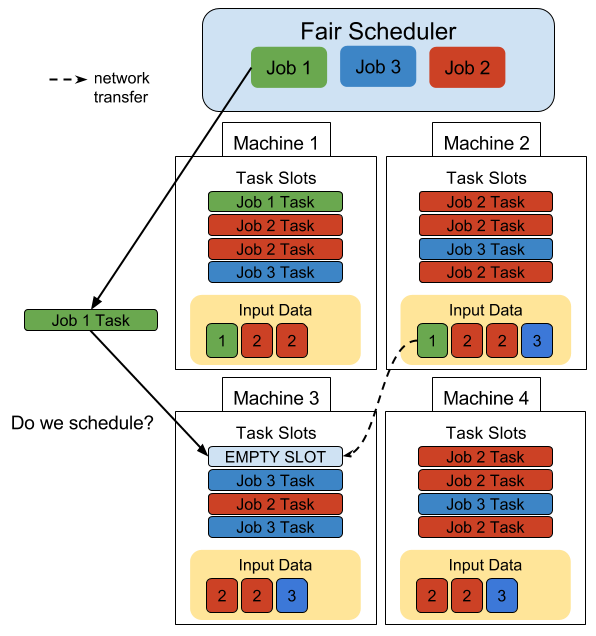
\includegraphics[width=\linewidth]{./fig1.png}
        \caption{A compute cluster, with a fair scheduler that must fill an empty slot}
        \label{fig:cluster}
    \endminipage
\end{figure}

The Hadoop Fair Scheduler (HFS)~\cite{Zaharia:EECS} is an influential example of a cluster framework 
scheduler that seeks to find this balance. The HFS was designed with two main goals: 
\textit{Fair sharing}: dividing resources using max-min fair sharing~\cite{Zaharia2008} to achieve 
statistical multiplexing, and 
\textit{Data locality}: placing computations (tasks) near their input data as often as
possible, to maximize system throughput. 

To achieve the first goal (fair sharing), a scheduler must reallocate resources between 
jobs when the number of jobs changes; however, a strict implementation of fair sharing 
compromises locality, because the job to be scheduled next according to fairness might not
have data on the nodes that are currently free. To resolve this problem, the HFS relaxes 
fairness slightly through a simple algorithm called 
\textit{delay scheduling}~\cite{Zaharia2010}, in which a 
job waits for a fixed amount of time for additional scheduling opportunities on nodes 
that have data for it, if none are available.

The original delay scheduling work~\cite{Zaharia2010} reported that a small amount of waiting is enough
to bring locality close to 100\% (the chosen default value is three seconds). Since its 
inception, delay scheduling has been used in other cluster framekwork schedulers, such as 
Spark, as well as in resource managers, such as YARN~\cite{Vavilapalli2013} and
Mesos~\cite{Hindman2011}.

Delay scheduling provides a simple solution for the scenario in 
Figure~\ref{fig:cluster}. Job 1 will simply be delayed for a fixed interval (and a task
from Job 3 scheduled in its place) in the hopes that data-local slots will open up in 
the future; however, delay scheduling assumes that data locality is always beneficial.
In reality, the decision is not as simple. The importance of data locality depends on many
factors, such as network conditions, input data size, disk i/o usage, and others. These
conditions may change over time (or even during the execution of a job). As well, with clusters
in the public cloud becoming so common, cluster conditions can change as simultaneous user
load changes, or after instances are stopped and restarted, potentially in a different physical
configuration. So, the
decision of whether or not to delay (and for how long) can not be efficiently solved with
a fixed, unchanging delay interval. We propose that an \emph{adaptive} mechanism is needed,
in order to properly judge and exploit these tradeoffs between fairness and locality,
based on feedback from the system.

In this paper, we present Dynamic Delay Scheduling, a simple, low-state, adaptive
solution for task scheduling in the cloud, which improves job latency over
fixed-interval delay scheduling. Dynamic Delay Scheduling operates by using feedback from finished
tasks in the system, which report their perceived overhead from remote data
reads. Our scheduler then adapts the delay scheduling interval to be used to schedule subsequent
tasks, using a running average of the overhead metrics reported as the interval
itself. In this way, our adaptive solution minimizes completion time by finding the shifting balance between:
1) immediate fairness policy enforcement, and 2) waiting for data locality, based on the severity of network overhead,
for increased performance.
This paper contributes an outline of this adaptive solution. We have
also implemented a simple prototype in Spark. Preliminary experiments demonstrate that
an adaptive delay outperforms the current Spark distribution (which uses a fixed delay
scheduling interval) in TPC-H workloads. 
%\textbf{Ideally, we need to identify some concrete statement concerning job latency and how it is minimized by DDS}

The remainder of this paper is structured in the following way. Section~\ref{sec:background}
presents background on fixed delay scheduling as a concept. Section~\ref{sec:systems} discusses how fixed delay
scheduling is implemented/mapped to real systems. Section~\ref{sec:dynamic} defines the terminology and
design of Dynamic Delay Scheduling, our simple adaptive scheduling solution. Section~\ref{sec:impl} describes our
lightweight implementation in Apache Spark. Section~\ref{sec:eval} demonstrates our evaluation of Dynamic
Delay Scheduling, using our implementation in Spark under several workloads. Finally, 
Section~\ref{sec:conclusion} provides closing remarks, and well as some future direction for further
applying adaptive algorithms to other facets of task scheduling.
%\textbf{Say a few words about expanding this work on adaptive algorithms}


\section{Delay Scheduling Background}\label{sec:background}

Delay scheduling is a heuristic designed to improve the data locality of tasks in the
context of fairness policy enforcement. We consider a cluster computing setting, where each 
application (or job), when submitted, is divided into many tasks which can be executed in 
parallel. The main components involved are: 1) a set of \textit{N} compute nodes, each with 
\textit{S} slots (one slot can run one task at a time), 2) a set of \textit{J} jobs, each 
with \textit{T} tasks, and 3) a set of \textit{D} blocks of data, distributed across the 
compute nodes, where each task in a job operates on one (specific) block.

To constitute fairness, each of the \textit{J} jobs must have an equal share of the 
cluster's resources. If there are 2 jobs, then each gets half of the cluster, if there 
are 3, then a third, etc. To implement this, a fair scheduler must maintain a sorted 
queue of the remaining jobs, based on their current share of the cluster. The job with 
the least running tasks (the job farthest below its fair share of resources) is at the 
head of this queue. Let us call this job \textit{J\_priority}. Tasks from this job will 
take priority over the rest in the queue.
   
An observation that can be made is that, when a compute slot opens up on one of the 
\textit{N} nodes, there might not be any data blocks on the node that the tasks of 
\textit{J\_priority} need. This is called \textit{data locality}. A task can 
be considered to be data local when it is scheduled in a slot on a node colocated with its
data. Fairness enforcement compromises data locality, because the next job in the 
scheduler's queue (based on fairness priority) might not have data in the next open slot 
in the cluster. Tasks that run non-locally must pull their input data in from across the 
network, causing an increase in completion time.

Traditional fixed delay scheduling operates in the following way: if 
\textit{J\_priority} does not have any data blocks it needs in the slot currently being 
considered, it will be temporarily skipped, and a task from a job further down the queue 
(a lower priority job) will be scheduled instead. \textit{J\_priority} will remain at the 
head of the queue (because it is still farthest below its fair share). 
\textit{J\_priority} will thus be the highest priority job for the next slot that opens 
up, which hopefully will have data it needs. After a finite number of failed scheduling 
attempts (skips), \textit{J\_priority} will be scheduled in the next open slot regardless 
of locality. The maximum number of skips is usually determined by the number of scheduling
attempts that occur within a certain interval of time (a few seconds). We can call this
interval of time the \textit{delay interval}.

The argument behind why fixed delay scheduling is acceptable is a probabilistic one. Assuming 
that slots free up frequently, the chance that an open slot will not overlap with a job's 
input data decreases exponentially. This chance is further decreased by block replication 
in distributed file systems (like HDFS), each of which can serve data for a task; however,
this probabilistic approach relies on both a) an equal probability of slots opening up on each machine across
the cluster, and b) a constant slot opening frequency. If the frequency were to change (for
example, if network conditions were to worsen and currently running tasks were to take longer to complete), 
then the chance of achieving locality during the same fixed interval decreases. As well,
variance in job profiles can lead to skewed probabilities of slot openings from machine
to machine (some tasks take
longer than others, some jobs have data on only a subset of machines, etc.). 

%\textbf{So? We need to complete this argument with a ``but'' to identify theoretically what can go wrong with constant delay scheduling}

%\textbf{Also, are we using delay scheduling to refer to ``constant'' delay scheduling by default?}


\section{Fixed Delay Scheduling in Cluster Frameworks}\label{sec:systems}

In real systems, fixed delay scheduling is usually implemented using a preset delay 
interval (as a unit of time, in milliseconds), and timestamps, the first of
which is taken the first time a job is considered for scheduling (whether a task is actually
scheduled or not).
This timestamp is checked whenever a slot opens. If the slot is on a machine
without input data for a job, then tasks from that job may only be scheduled there if
the time between the current time and the timestamp is greater than whatever the fixed delay
interval is. If the slot \textit{does} have input data for the job, then tasks can be scheduled
no matter the timestamp. Regardless of how/why a task was scheduled for a job, once a task
is scheduled then the timestamp is reset, and the process begins again. Very little extra
state is required (just one additional field for each job currently in progress). For the purposes
of this paper, we will be focusing on how fixed delay scheduling operates in Apache Spark (detailed
below), but the principles and implementations are the same in other systems, such as 
Hadoop, YARN, and Mesos.

Apache Spark [ref] is a general execution engine for distributed "Big Data" processing, 
similar to Hadoop, that breaks jobs into stages of tasks, and uses fixed delay scheduling to 
improve data locality when launching these tasks. Spark provides many advantages, such 
as an abstraction for representing distributed datasets (Resilient Distributed Datasets, 
or RDDs). These RDDs, which represent data either on disk (in Hadoop Distributed File 
System, or HDFS) or in memory, are divided into partitions across worker processes called 
executors in the cluster. Each executor has a finite number of slots (usually equal to the number 
of CPU cores available) with which to run 
tasks. The Spark scheduler, which resides in a centralized driver process separate from 
the executors, uses fixed delay scheduling to provide greater data locality when scheduling 
tasks into slots that become open. The fixed delay interval (the maximum waiting time) is set 
statically in a configuration file.

Spark (and the other systems mentioned above) also provide hierarchical fixed delay scheduling.
That is, a delay interval can be specified for each node-local, rack-local, or even datacenter-local
scheduling. If the delay interval expires for a job, rather than being scheduled, it will fall back
into the next tier, and delay there (for perhaps a different period of time than the original interval)
for slots with the relaxed locality condition of that tier (slots within the same rack as input data, for
example). 



\section{Dynamic Delay Scheduling}\label{sec:dynamic}

\subsection{Beyond Constant Delays}

The frameworks described above use a fixed delay interval, 
which remains the same throughout an entire job. Our observation is that there is a 
calculable tipping point after which waiting/skipping is no longer beneficial. Generally,
we can define the total running time of a task \textit{t} as:

\[
t\_total = t\_compute + t\_netOH + sch\_delay
\]

where \textit{t\_compute} is the local computation time of the task, \textit{t\_netOH}
is the network latency incurred from data transfer (this is zero if the task is scheduled 
locally), and \textit{sch\_delay} is the amount of time \textit{t} is delayed 
(skipped) to wait for locality, from the moment \textit{t} is first considered for 
scheduling.

Ideally, we want to minimize the task completion time of all tasks within a given job, 
while also providing some guarantee as to the maximum latency introduced by the scheduler
itself through delay scheduling. The goal of delay scheduling is to remove \textit{t\_netOH} by 
scheduling a task locally, but if the task is delayed longer than this \textit{t\_netOH}, 
then it would have actually been more efficient in hindsight (in terms of task completion time) 
to immediately schedule the task in the first open slot that was considered. 
Conversely, if the delay interval is too short, then the task could potentially miss 
scheduling opportunities with locality, which would result in a shorter completion time
than scheduling without locality.

Dynamic Delay Scheduling improves upon fixed delay 
scheduling by dynamically adapting the maximum 
\textit{sch\_delay} equal to \textit{t\_netOH} on a per-task basis. This allows 
for the longest waiting time for data-local slots while limiting the worst case task 
running time to \textit{t\_compute + (2 * t\_netOH)}. In this way, the delay interval
will adapt to the severity of the network overhead. If \textit{t\_netOH} is low, then locality
is less of a concern and the scheduler can shorten the time it delays. If \textit{t\_netOH} becomes high,
then the scheduler increases the time that it waits, as locality is more important in poorer network
conditions; however, this means that the 
network overhead incurred by running tasks needs to be monitored and reported to the 
scheduler over time, in order to adapt to changing network conditions and potentially 
heterogeneous data block sizes. 

\subsection{An Adaptive Solution Using Task Feedback}

The network overhead incurred by missing data locality depends on many factors, including 
network traffic, the distance of a task from its data, and the input data size. These 
factors vary from job to job, and some (like network traffic) can change during the job 
execution itself. In order to adapt the delay scheduling interval to changing conditions, 
we have designed a simple feedback mechanism, in which each task reports the network overhead it experienced 
upon completion (\textit{t\_netOH}, for a task \textit{t}). This metric is sent to a 
centralized fair scheduler, which then changes its delay scheduling interval using a 
running average of feedback from completed tasks. This new delay scheduling interval is 
then used when scheduling subsequent tasks of the same type.

The feedback metric itself (\textit{t\_netOH}) can be any time measurement which 
reflects the network overhead incurred by a task. In the case of Dynamic Delay Scheduling, we are 
considering tasks which read data from distributed file systems,
so the \textit{t\_netOH} for each task is the amount of time spent 
reading data blocks remotely; however, any arbitrary type of task, which has some way of 
measuring its own overhead, could set this as well and benefit from the adaptation.

%\newcommand{algrule}[1][.2pt]{\par\vskip.5\baselineskip\hrule height #1\par\vskip.5\baselineskip}

\begin{algorithm}[]
    \footnotesize
    \DontPrintSemicolon
    \caption{Dynamic Delay Scheduling}
    \textbf{Initialization:}\;
    delay\_interval $\leftarrow$ default (3 seconds)\;
    \hrule width 0.4\textwidth
    \;
    \textbf{Upon receiving task $t$ completion event:}\;
    delay\_interval $\leftarrow$ (delay\_interval + t\_netOH) / 2\;
    \hrule width 0.4\textwidth
    \;
    \textbf{Scheduling Procedure:}\;
    \For{each open slot $s$ on a node $n$ in N}{
        sort $J$ in increasing order of currently running tasks\;
    
        \For{$j$ in $J$}{
            \If{$j$ has just launched a task}{
                $j$.wait\_begin = current\_time\;
            }
            \eIf{a task $t$ in $j$ has data on $s$'s node $n$}{
                launch t in $s$\;
            }{
                \If{a task $t$ in $j$ is unlaunched}{
                    \eIf {current\_time - $j$.wait\_begin $>$ delay\_interval}{
                        launch $t$ in slot $s$\;
                    }{
                        continue\;
                    }
                }
            }
        }
    }
\end{algorithm}


Algorithm 1 describes our adaptive solution in detail, in a cluster with \textit{N} nodes and \textit{J} jobs. 
When tasks complete, the delay interval will be changed to reflect 
recent overhead measurements. The delay interval adapts relatively quickly (the average of
the last few readings), since feedback can only be received when tasks complete. For workloads
in which tasks complete very often, the window for the average can be broadened. 
During scheduling, this new interval is used for delay scheduling (and this interval can 
change even while a job is currently waiting, as tasks complete). It is worth noting that 
there is nothing preventing this adaptive solution from also being hierarchical, as many 
frameworks desire/implement separate delay intervals for node-local or rack-local scheduling.


\section{Implementation in Spark}\label{sec:impl}

We have implemented Dynamic Delay Scheduling in Spark, for tasks which read data
from HDFS as input.
Our implementation consists of about 100 lines of Scala code, which modify the
already-existing fixed delay scheduling mechanisms as well as store a small bit
of extra state.

The \textit{t\_netOH} for each task is implemented as a new field in 
each TaskContext, called \textit{netOH}. To compute the overhead, we have inserted a 
wrapper for the HDFS RecordReader, which sums reading time. When a task completes, it 
will set \textit{netOH} to this sum, and then send it back to the Spark scheduler via the 
event bus that drives the system. While we have focused our implementation on ``map-like'' 
tasks which read from HDFS (which have predictable behavior), any arbitrary task could 
monitor its own overhead and set this field before closing.

The Spark Scheduler, when it sees a TaskCompleted event, will pull off that task's 
\textit{netOH} and average it into a global \textit{delay\_interval} that is used for all 
tasks in the same ``stage'' (stages are groups of tasks which do the same thing). Then, 
when a slot opens up in the cluster, the most recent \textit{delay\_interval} will be 
used in place of the delay interval fetched from the spark-defaults.conf file. 

Finally, we note that our implementation is simple enough to be adapted to other frameworks
that use delay scheduling as well, as most systems (such as Hadoop) also have events/messages
that inform the scheduler with information about finished tasks.



\section{Evaluation}\label{sec:eval}

In order to test the efficiency of Dynamic Delay Scheduling, we have designed several 
tests, on both a small and a large scale, using our implementation in Spark, with fair
scheduling enabled. The goal of
these experiments is to demonstrate that an adaptive delay interval provides decreased
job latency in a variety of cluster setups and workloads.

\subsection{Evaluation Setup}
Our small-scale tests were performed on a four node local cluster, with four
task slots (four 1.6 GHz cores for Spark tasks) per machine. All four nodes were
connected through a Gigabit Ethernet switch. The workload chosen for the
small-scale test was an integer sort, on 1GB of input data spread across HDFS.
The main goal behind the small-scale setup is to evaluate our algorithm in a
controlled environment with stable network conditions. To provide data locality
concerns, input data was placed on two nodes, so as to ensure both data-local
and non-local slots for task placement.

In order to have a more realistic evaluation, our large-scale tests were
performed on a 16 node cluster on Amazon EC2, using m3.xlarge instances. The
workload chosen for the large scale test was a TPC-H benchmark (\#7), which
performs a query reading from multiple databases in HDFS, of size ranging from
several megabytes to 80 gigabytes (for a total of ~120GB of input data).
The benchmark is designed to simulate a business query determining the value of
goods shipped between two countries. We chose this particular benchmark because
it consists of a mixture of large and small stages which read from these tables
in parallel. This causes contention for resources in the cluster, creating
situations in which locality and fairness clash. This benchmark also represents
a workload in which fairness is likely to be desired. Without fair sharing,
stages which read from small tables would be significantly delayed by
longer-running stages operating on larger data sets.
All numbers, from both small and large scale, are the average of 3 runs, with
error bars shown.

\subsection{Small Scale Results}
\masoud{@Derek: Argue why sort is a good application for our controlled small
scale eval} The results of our small-scale tests are shown in Figure~\ref{fig:smallscale}.
We performed the sort with the default fixed delay interval (fixed 3 seconds),
with dynamic delay scheduling, and with no delay for comparison. The default of
3 seconds causes a slight increase in completion time (versus no delay). Given
that network conditions were very good between the nodes in the cluster (all
connected to the same switch), having a fixed delay value of 3 seconds causes
increased overhead, because the network overhead of missing locality is far
shorter than 3 seconds. Our adaptive solution performs slightly better, because
the delay interval shrinks based on the feedback from the first round of tasks,
although the job is still too small for there to be the kind of resource
contention that would result in larger speedups. This experiment simply
demonstrates that an incorrect fixed delay interval can actually hurt the
performance of a job, rather than improve it.

\subsection{Large Scale Results}

The results of our large-scale TPC-H tests are shown in Figure~\ref{fig:largescale}, with the same three 
delay setups (fixed 3 seconds, our dynamic solution, and no delay). Even though the default
value still improves completion time versus no delay, the dynamic solution outperforms 
the fixed delay by 15\%. Since the dynamic solution eliminates extraneous
waiting while also still providing an appropriate time to wait for data locality, we see
an improvement over the fixed delay. The improvement is larger than the small-scale for
several reasons. First, with this test being performed in the cloud, network guarantees
are not as strong, creating the need for adaptability if network conditions change. 
Second, with this being a large workload with hundreds of tasks, there is greater 
contention for slots amongst all running stages, creating more opportunity for delay 
scheduling to be applied.

\begin{figure}[t]
    \minipage{0.5\textwidth}
        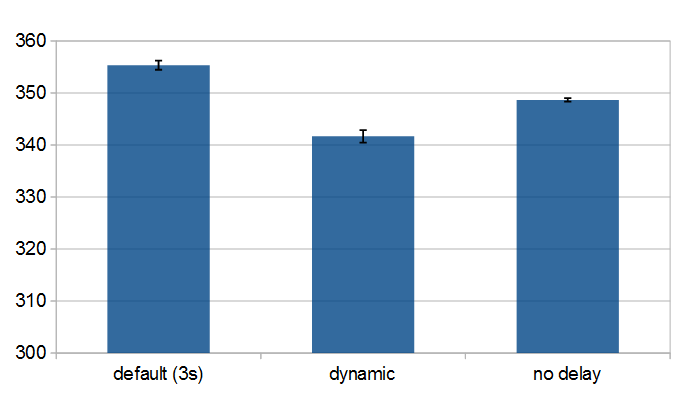
\includegraphics[width=\linewidth]{./smallscale.png}
        \caption{1GB Spark Sort - Job Completion Time (s) vs. Delay Type}
        \label{fig:smallscale}
    \endminipage \hfill
\end{figure}

\begin{figure}[t]
    \minipage{0.5\textwidth}
        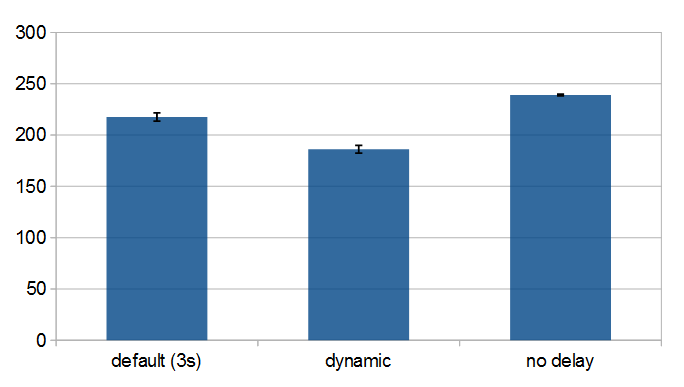
\includegraphics[width=\linewidth]{./largescale.png}
        \caption{120GB Spark TPC-H Query - Job Completion Time (s) vs. Delay Type}
        \label{fig:largescale}
    \endminipage \hfill
\end{figure}




\section{Conclusion}\label{sec:conclusion}

Delay scheduling has long been accepted as a \textit{de facto} solution for achieving
higher data locality (and assumedly better performance) in cluster framework schedulers that
enforce fairness. We show that 
delay scheduling, using a fixed delay interval, is inefficient, and can be improved by 
adapting the delay interval on-the-fly, based on the overhead experienced by completed tasks. 
An adaptive solution allows delay scheduling to find a proper balance between fairness and
performance, based on changing network conditions, job profiles, and cluster usage.

Regarding future work, there are other areas where adaptivity looks promising in the realm of
delay scheduling. For example, the frequency with which tasks complete is major contributor
to the probability that delay scheduling will actually provide locality, and could potentially
be used as another adaptive improvement. Other feedback metrics (such as task completion time) 
hold promise for improvements as well. Finally, avenues exist for optimally creating 
schedules of tasks (rather than the greedy scheduling currently used), assuming enough accurate
real-time feedback can be gained from running (or about to run) jobs. 





%
%\thispagestyle{empty}
%\clearpage
\pagenumbering{arabic}
%
\bibliography{references}

\end{document}

%%% Local Variables:
%%% mode: latex
%%% TeX-master: t
%%% End:
